\begin{figure}
\centering
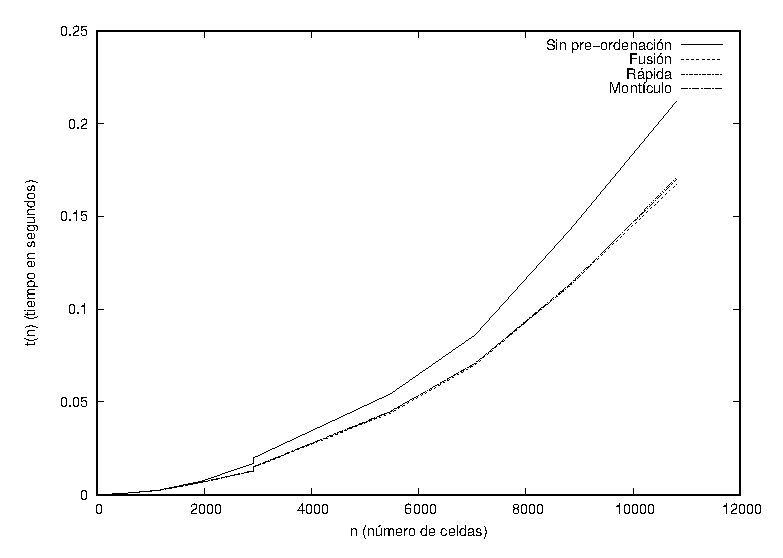
\includegraphics[width=0.7\linewidth]{./graphic.eps} % no es necesario especificar la extensión del archivo que contiene la imagen
\caption{Estrategia devoradora para la mina}
\label{fig:Grafica}
\end{figure}

\begin{lstlisting}
#define BUILDING_DEF_STRATEGY_LIB 1

#include "../simulador/Asedio.h"
#include "../simulador/Defense.h"
#include "cronometro.h"

using namespace Asedio;     

//funcion encargada de calcular la distancia ente dos objetos dando de estos su posicon y su radio
float distObjeRad(Vector3 posicion1, float radio1, Vector3 posicion2, float radio2) {

    float dist = _distance(posicion1, posicion2) - (radio1 + radio2);
    if (dist < 0) { // Caso en que los obstaculos chocan
        return 0; 
    }
    else{
        return dist;
    }
}

float defaultCellValue(int row, int col, bool** freeCells, int nCellsWidth, int nCellsHeight               
    , float mapWidth, float mapHeight, List<Object*> obstacles, List<Defense*> defenses) {
    	
    float cellWidth = mapWidth / nCellsWidth;
    float cellHeight = mapHeight / nCellsHeight;

    Vector3 cellPosition((col * cellWidth) + cellWidth * 0.5f, (row * cellHeight) + cellHeight * 0.5f, 0);
    	
    float val = 0;
    for (List<Object*>::iterator it=obstacles.begin(); it != obstacles.end(); ++it) {
	    val += _distance(cellPosition, (*it)->position);
    }

    return val;
}

bool factible(Object* defensa, int row, int col, int cellH, int cellW, float mapWidth, float mapHeight, List<Object*> obstacles, List<Defense*> defenses) {
    
    
    auto cell = Vector3(row * cellH + cellH * 0.5f, col * cellW + cellW * 0.5f, 0);
    bool res = true;
    if ((defensa->radio >= cell.x || cell.x >= mapWidth - defensa->radio) || (defensa->radio >= cell.y || cell.y >= mapHeight - defensa->radio) ) {
        res = false;
    }
    for (auto it = obstacles.begin(); it != obstacles.end() && res; it++){
        if (distObjeRad(cell, defensa->radio, (*it)->position, (*it)->radio) <= 5) {
            res = false;
        }
    }
    for (auto it = defenses.begin(); it != defenses.end() && res; it++){
        if (distObjeRad(cell, defensa->radio, (*it)->position, (*it)->radio) <= 0) {
            
            res = false;
        }
        
    }
    return res;   
}

void quicksort(float* vec,int pri,int ult)
{
    int med = (pri+ult)/2, i = pri, j = ult;
    double pivote = vec[med];

    do{   
        while(vec[i] > pivote) { i++; }
        while(vec[j] < pivote) { j--; }
        if(i<=j){
            int aux = vec[i];
            vec[i] = vec[j];
            vec[j] = aux;
            i++;
            j--;
        }
    } while(i <= j);
    if(pri < j)
        quicksort(vec, pri, j); /*mismo proceso con sublista izquierda*/
    if( i< ult)
        quicksort(vec, i, ult); /*mismo proceso con sublista derecha*/
}

void merge(float* vec, int tam, int izquierda, int medio, int derecha){
    int h = izquierda ,i = izquierda ,j = medio + 1;
    float res[tam];
    
    while((h <= medio) && (j <= derecha)){
        if(vec[h] >= vec[j]){
            res[i] = vec[h];
            h++;
        }
        else{
            res[i] = vec[j];
            j++;
        }
        i++;
    }
    if(h > medio){
        for(int k = j; k <= derecha; k++){
            res[i] = vec[k];
            i++;
        }
    }
    else{
        for(int k = h; k<=medio; k++){
            res[i] = vec[k];
            i++;
        }
    }
    for(int k = izquierda; k<=derecha; k++){
        vec[k] = res[k];
    }
}

void merge_sort(float* vec, int tam, int izquierda, int derecha){
    if(izquierda>derecha){
        int medio=(izquierda+derecha)/2;
        merge_sort(vec, tam, izquierda, medio);
        merge_sort(vec, tam, medio+1, derecha);
        merge(vec, tam, izquierda, medio, derecha);
    }
}

void DEF_LIB_EXPORTED placeDefenses3(bool** freeCells, int nCellsWidth, int nCellsHeight, float mapWidth, float mapHeight
              , List<Object*> obstacles, List<Defense*> defenses) {

    float cellWidth = mapWidth / nCellsWidth;
    float cellHeight = mapHeight / nCellsHeight; 
    int tam = nCellsHeight * nCellsWidth;
    float ErrRel = 0.001;
    float ErrAbs = 0.01;
    float Err = ErrAbs * ErrRel + ErrAbs;

    cronometro A, B, C, D;
    int ra = 0, rb = 0, rc = 0, rd = 0;

    A.activar();
    do {
        ra++;
        float* cellValues = new float[tam]; 
        for(int i = 0; i < nCellsHeight; ++i) {
            for(int j = 0; j < nCellsWidth; ++j) {
                cellValues[i * nCellsHeight +j] = defaultCellValue(i, j, freeCells, nCellsWidth, nCellsHeight, mapWidth, mapHeight, obstacles, defenses);
            }
        }

        auto defAct = ++defenses.begin();
        int i = 0;
        bool fin1 = true;
        while (defAct != defenses.end()){
            while (fin1 && cellValues[i] != cellValues[nCellsHeight + nCellsWidth - 1]){
                if ( cellValues[i] != NULL && factible(*defAct, i / nCellsWidth, i % nCellsWidth, cellHeight, cellWidth, mapWidth, mapHeight, obstacles, defenses)){
                    (*defAct)->position = Vector3(i / nCellsWidth * cellHeight + cellHeight * 0.5f, i % nCellsHeight * cellWidth + cellWidth * 0.5f, 0);;
                    fin1 = false;
                    cellValues[i] = NULL;
                    i = 0;
                }
                else{
                    i++;
                }
            }
            fin1 = true;
            defAct++;
        }
    }while (A.tiempo() < Err);
    A.parar();

    B.activar();
    do {
        rb++;
        float* cellValues = new float[tam]; 
        for(int i = 0; i < nCellsHeight; ++i) {
            for(int j = 0; j < nCellsWidth; ++j) {
                cellValues[i * nCellsHeight +j] = defaultCellValue(i, j, freeCells, nCellsWidth, nCellsHeight, mapWidth, mapHeight, obstacles, defenses);
            }
        }

        merge_sort(cellValues, tam, 0, tam-1);

        auto defAct = ++defenses.begin();
        int i = 0;
        bool fin1 = true;
        while (defAct != defenses.end()){
            while (fin1 && cellValues[i] != cellValues[nCellsHeight + nCellsWidth - 1]){
                if ( cellValues[i] != NULL && factible(*defAct, i / nCellsWidth, i % nCellsWidth, cellHeight, cellWidth, mapWidth, mapHeight, obstacles, defenses)){
                    (*defAct)->position = Vector3(i / nCellsWidth * cellHeight + cellHeight * 0.5f, i % nCellsHeight * cellWidth + cellWidth * 0.5f, 0);;
                    fin1 = false;
                    cellValues[i] = NULL;
                    i = 0;
                }
                else{
                    i++;
                }
            }
            fin1 = true;
            defAct++;
        }
    }while (B.tiempo() < Err);
    B.parar();

    C.activar();
    do {
        rc++;
        float* cellValues = new float[tam]; 
        for(int i = 0; i < nCellsHeight; ++i) {
            for(int j = 0; j < nCellsWidth; ++j) {
                cellValues[i * nCellsHeight +j] = defaultCellValue(i, j, freeCells, nCellsWidth, nCellsHeight, mapWidth, mapHeight, obstacles, defenses);
            }
        }

        quicksort(cellValues, 0, tam-1);

        auto defAct = ++defenses.begin();
        int i = 0;
        bool fin1 = true;
        while (defAct != defenses.end()){
            while (fin1 && cellValues[i] != cellValues[nCellsHeight + nCellsWidth - 1]){
                if ( cellValues[i] != NULL && factible(*defAct, i / nCellsWidth, i % nCellsWidth, cellHeight, cellWidth, mapWidth, mapHeight, obstacles, defenses)){
                    (*defAct)->position = Vector3(i / nCellsWidth * cellHeight + cellHeight * 0.5f, i % nCellsHeight * cellWidth + cellWidth * 0.5f, 0);;
                    fin1 = false;
                    cellValues[i] = NULL;
                    i = 0;
                }
                else{
                    i++;
                }
            }
            fin1 = true;
            defAct++;
        }
    }while (C.tiempo() < Err);
    C.parar();

    D.activar();
    do {
        rd++;
        float* cellValues = new float[tam]; 
        for(int i = 0; i < nCellsHeight; ++i) {
            for(int j = 0; j < nCellsWidth; ++j) {
                cellValues[i * nCellsHeight +j] = defaultCellValue(i, j, freeCells, nCellsWidth, nCellsHeight, mapWidth, mapHeight, obstacles, defenses);
            }
        }

        std::make_heap(cellValues, cellValues + tam - 1);

        auto defAct = ++defenses.begin();
        int i = 0;
        bool fin1 = true;
        while (defAct != defenses.end()){
            while (fin1 && cellValues[i] != cellValues[nCellsHeight + nCellsWidth - 1]){
                if ( cellValues[i] != NULL && factible(*defAct, i / nCellsWidth, i % nCellsWidth, cellHeight, cellWidth, mapWidth, mapHeight, obstacles, defenses)){
                    (*defAct)->position = Vector3(i / nCellsWidth * cellHeight + cellHeight * 0.5f, i % nCellsHeight * cellWidth + cellWidth * 0.5f, 0);;
                    fin1 = false;
                    cellValues[i] = NULL;
                    i = 0;
                }
                else{
                    i++;
                }
            }
            fin1 = true;
            defAct++;
        }
    }while (D.tiempo() < Err);
    D.parar();

    std::cout << (nCellsWidth * nCellsHeight) << '\t' << A.tiempo() / ra << '\t' << B.tiempo() / rb << '\t' << C.tiempo() / rc << '\t' << D.tiempo() / rd << std::endl;
}
\end{lstlisting}